%
% 第五章
%
\chapter{硬盘文件安全加载方案实现及测试}
有了三四章节的理论和代码基础,本章将在此基础上,逐步进行实验验证分析。验证内容包括,DXE阶段驱动程序度量功能
的验证、BDS阶段硬盘文件度量功能的验证、UEFI系统中BMC驱动程序的连通性验证、通过EDKII编译生成的fd固件文件格式
的验证以及DXE阶段修改驱动程序加载顺序的验证。下面将先对实验环境进行介绍,以及选用的原因。

%
% 5.1节
%
\section{实验环境}

\subsection{申威6A服务器真机环境}
实验的真机环境是可信固件实验室提供的申威6A型服务器,实验环境包括了固件的编译环境以及服务器中BMC提供的fd固件
文件烧写环境,具体信息如下:
\par (1)固件编译系统环境:Ubuntu 10.04版本,并配置uuid-dev-2.17包
\par (2)固件编译工具:原版gcc4.4.3,和申威定制的swgcc-4.5.3-交叉编译器
\par (3)EDKII信息:带有申威定制包SenweiPkg的EDKIIR13995版本
\par (4)BMC烧写环境:Ubuntu 16.04版本和Firefox浏览器
\par Ubuntu 10.04版本的选择主要原因在于它提供的C语言库函数版本问题,由于swgcc-4.5.3-交叉编译器的特殊性,
需要特定库版本的支持,在以往实验中这一点经过验证。由于真机环境上运行的固件是经过申威ALPHA64架构处理器指令集定
制的,因此根据编译环境的特殊性做一些编译方法的介绍。交叉编译器的设置是通过linux系统软链接的方式实现的:

\begin{lstlisting}
    ln -s sw_64sw2-unknown-linux-gnu-ar swar
    ln -s sw_64sw2-unknown-linux-gnu-as swas
    ln -s sw_64sw2-unknown-linux-gnu-gcc swgcc
    ln -s sw_64sw2-unknown-linux-gnu-ld swld
    ln -s sw_64sw2-unknown-linux-gnu-objcopy swobjcopy    
\end{lstlisting}

通过以上命令分别将申威定制版本的gcc编译器链接到官方版本gcc的调用名称上面,来实现编译命令的调用。

\begin{figure}[htb]
    % 调整图片与上文的垂直距离 %
    \vspace{0cm}   
    % 调整图片图片与中文标题、中文标题与英文标题距离 %
    \setlength{\abovecaptionskip}{0.3cm}
    % 引用/fig/目录中的图片文件 %
	\centering
    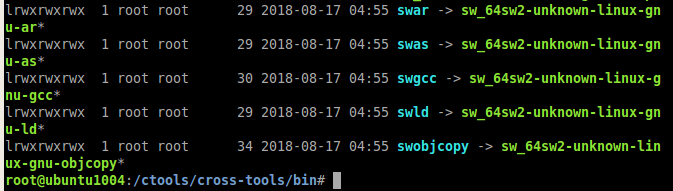
\includegraphics[width=12cm]{cross_tools.png}
    % 中文标题 %
    \caption*{图 5-1 编译器软连接}
    % 调整图片英文标题与下文距离(本文标准为-0.7cm) %
    \setlength{\belowcaptionskip}{-0.5cm}
    % 英文标题 %
    \caption*{Fig.5-1 Compiler Soft Link}
\end{figure}

图5-1所示的是查看软链接的修改效果。接下来是交叉编译申威固件程序的过程,首先需要使用原版gcc4.4.3编译器进行
edksetup程序的初始化工作,这个程序的目的在于为正在打开着的终端窗口设置好通过build编译时一切所需的环境变量
及一些通过C语言根据UEFI规范自动生成的代码内容。

\begin{figure}[htb]
    % 调整图片与上文的垂直距离 %
    \vspace{0cm}   
    % 调整图片图片与中文标题、中文标题与英文标题距离 %
    \setlength{\abovecaptionskip}{0.3cm}
    % 引用/fig/目录中的图片文件 %
	\centering
    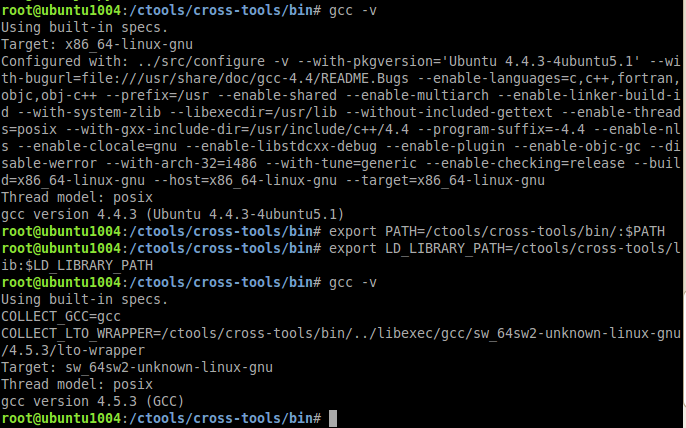
\includegraphics[width=12cm]{swgcc.png}
    % 中文标题 %
    \caption*{图 5-2 GCC版本切换过程}
    % 调整图片英文标题与下文距离(本文标准为-0.7cm) %
    \setlength{\belowcaptionskip}{-0.7cm}
    % 英文标题 %
    \caption*{Fig.5-2 GCC version switching process}
\end{figure}

如图5-2所示,是通过export改变环境变量的命令,将我们设置好的swgcc交叉编译器软链接目录添加到两个系统环境
变量中的过程,通过这样的方式,就可以实现用gcc 4.4.3版本进行edksetup程序的运行,并用swgcc交叉编译器进行
平台dsc文件的构建编译过程。具体编译过程,采用linux SHELL脚本的方式进行使用,如图下代码所示。

\begin{lstlisting}
    cd dev
    cd uefibasic
    . edksetup.sh
    export PATH=/ctools/cross-tools/bin/:$PATH
    export LD_LIBRARY_PATH=/ctools/cross-tools/lib:$LD_LIBRARY_PATH
    cd SenweiPkg
    . build.sh
\end{lstlisting}

% \begin{figure}[H]
%     % 调整图片与上文的垂直距离 %
%     \vspace{0cm}   
%     % 调整图片图片与中文标题、中文标题与英文标题距离 %
%     \setlength{\abovecaptionskip}{0.3cm}
%     % 引用/fig/目录中的图片文件 %
% 	\centering
%     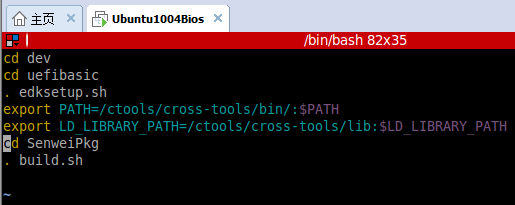
\includegraphics[width=12cm]{sw_sh_file.png}
%     % 中文标题 %
%     \caption*{图 5-3 交叉编译功能的终端程序}
%     % 调整图片英文标题与下文距离(本文标准为-0.7cm) %
%     \setlength{\belowcaptionskip}{-0.7cm}
%     % 英文标题 %
%     \caption*{Figure 5-3 Cross compile shell program}
% \end{figure}

\begin{figure}[htb]
    % 调整图片与上文的垂直距离 %
    \vspace{0cm}   
    % 调整图片图片与中文标题、中文标题与英文标题距离 %
    \setlength{\abovecaptionskip}{0.3cm}
    % 引用/fig/目录中的图片文件 %
	\centering
    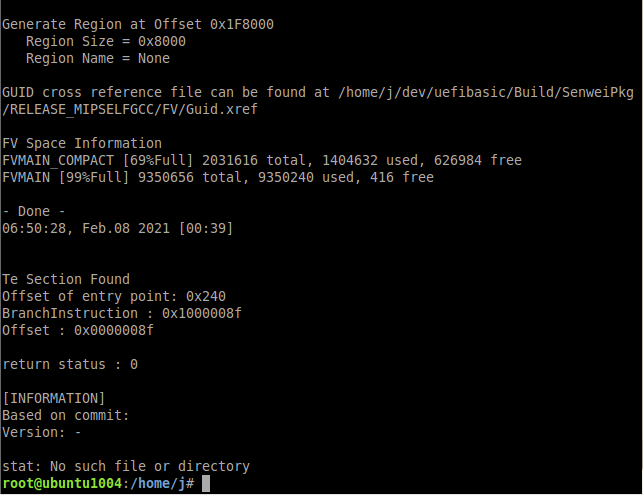
\includegraphics[width=12cm]{compile_res.png}
    % 中文标题 %
    \caption*{图 5-3 交叉编译结果}
    % 调整图片英文标题与下文距离(本文标准为-0.7cm) %
    \setlength{\belowcaptionskip}{-0.4cm}
    % 英文标题 %
    \caption*{Fig.5-3 Cross compile result}
\end{figure}

其中的实现为开发的脚本语言编译程序,图5-4为最终的固件编译结果。

% \subsection{UEFI Windwos模拟环境}
% 与真机环境对应的是Windows系统下的UEFI模拟运行环境,建立这个环境的目的在于,能够简化固件开发过程中调试的
% 复杂程度,通过模拟环境测试一些硬件结构不相关的功能模块运行效果,增加开发效率。其中具体信息如下:
% \par (1)固件编译系统环境:Windows 10
% \par (2)固件编译工具:VS2008
% \par (3)EDKII信息:EDKIIR13995版本
% \par 模拟环境的编译较为简单因此不做详细说明,编译效果图如图5-5。其中是GenFds命令生成最终fd固件文件的过程,
% 固件名称为NT32.fd。

% \begin{figure}[htb]
%     % 调整图片与上文的垂直距离 %
%     \vspace{0cm}   
%     % 调整图片图片与中文标题、中文标题与英文标题距离 %
%     \setlength{\abovecaptionskip}{0.3cm}
%     % 引用/fig/目录中的图片文件 %
% 	\centering
%     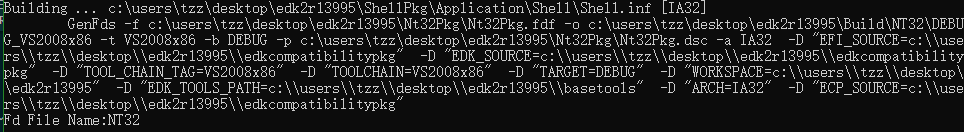
\includegraphics[width=12cm]{win_compile.png}
%     % 中文标题 %
%     \caption*{图 5-5 UEFI模拟环境编译结果}
%     % 调整图片英文标题与下文距离(本文标准为-0.7cm) %
%     \setlength{\belowcaptionskip}{-0.7cm}
%     % 英文标题 %
%     \caption*{Figure 5-5 UEFI simulation environment compilation results}
% \end{figure}

%
% 5.2节
%
\section{驱动度量功能实现与测试}
本文中在DXE阶段加载的可信度量驱动程序,主要用来度量四个UEFI文件系统协议栈驱动程序,并向BMC发送度量日志。
基于以上功能对可信度量驱动程序进行功能开发与测试。

\subsection{功能实现}
驱动度量函数首先根据传进来的内存中的驱动数据结构表示,判别驱动类型,由于四个文件系统协议栈驱动都属于
EFI\_IMAGE\_SUBSYSTEM\_EFI\_RUN-\newline TIME\_DRIVER类型\cite{addition3},因此可以通过这个条件进行初步判断。
在确定驱动类型正确
之后,进行GUID的判别,其中的四个特定驱动程序GUID通过INF文件获取的方式写死在代码中。若确定此正在加载的驱动
是四个驱动之一,则通过可信度量值计算模块中的SHA1计算协议进行度量,并通过GUID在BMC中获取到相应的基准值,
这些功能都通过BmcCheck函数实现。

\begin{lstlisting}
    EFI_STATUS
    DriverMeasurement(
        IN LOADED_IMAGE_PRIVATE_DATA   *Image
    ) {
        switch (Image->ImageContext.ImageType) {
        ...
        case EFI_IMAGE_SUBSYSTEM_EFI_RUNTIME_DRIVER:
            if (CompareGuid(Image->ImageContext->Name, DiskIoDxeName) ||
                CompareGuid(Image->ImageContext->Name, PartitionDxeName) ||
                CompareGuid(Image->ImageContext->Name, AtaAtapiPassThruDxeName) ||
                CompareGuid(Image->ImageContext->Name, FatFileSysName))
                    BmcCheck(Image->ImageContext);
        ...
    }
\end{lstlisting}
\par GUID匹配具体通过编写的CompareGuid函数比较128位的GUID值,通过把128位的GUID数据结构通过强制类型转换
(CONST UINT64*) Guid转换为UEFI系统中可以直接通过==符号进行比较的UINT64数据类型的指针,指针中包含了两个
元素,分别是GUID的高64位和底64位,然后通过表达式
(LowPartOfGuid1 == LowPartOfGuid2 \&\& HighPartOfGuid1 == HighPartOfGuid2)来返回比较结果的BOOLEAN
类型值。
\begin{lstlisting}
UINTN
EFIAPI
SerialPortWrite (
    IN UINT8     *Buffer,
    IN UINT32     Size
    )
{
    PRINTCONFIG* Pconfig;
    UINT8 cpuid;
    cpuid = hard_smp_processor_id ();
    cpuid = cpuid & (CORENUM_PER_CG - 1);
    Pconfig = PRINTK_BUF_CONFIG;
    Pconfig += cpuid;
    ...
    CopyMem (Pconfig->Start + Pconfig->Index, Buffer, Size);
    Pconfig->Index += Size;
    ...
}
\end{lstlisting}
上述代码描述的是度量日志写入功能中向串口写入信息的函数。其中输入参数Buffer是使用系统调用AsciiVSPrint函数
后,通过DEBUG信息生成的ASCII码格式的字符串,用8位的无符号整数的指针表示,其中每8位正好对应一个ASCII码,
表示一个英文字符。PRINTCONFIG是一个用来在内存中表示打印信息参数的数据结构,用于记录每次Buffer需要写入的
目的地址,其中Start字段是PRINTCONFIG在内存中的起始地址,Index字段用于在每次写入以此Buffer数据后,自加一
以达到下次调用串口写入函数时,写入到上次数据内容的后面。PRINTCONFIG的地址是通过计算得到的,PRINTK\_BUF\_CONFIG
是一个系统写死的数值,内容为0xfffffc0000870000UL,用于记录PRINTCONFIG结构在IO映射地址的位置,此内容是
在系统DXE阶段初始化过程中确定的。

\subsection{测试目的}
该可信度量功能对DXE阶段特定驱动的度量方法存在普遍性,给出了根据现有UEFI驱动加载的设计理念,自定义度量驱动
内容的方法。该过程的正确性直接影响了BDS阶段加载硬盘文件的安全可信性。

\subsection{测试步骤}
(1)首先编写具有上述五个模块的DXE阶段可信度量驱动程序,并将其模块INF文件通过引用的方式添加到将要编译的申威平台
描述文件dsc文件中。
\par (2)然后通过本章第一节中的方法,对申威UEFI组件进行交叉编译。
\par (3)通过BMC芯片提供的网卡端口服务程序,用单独的客户端主机访问服务器上的网卡端口,此过程设置客户端
静态IP,设置成与BMC提供的服务IP同一网段内,并烧写UEFI BIOS固件文件到服务器的闪存芯片中。
\par (4)服务器上电并按电源按钮,进入UEFI BIOS启动流程,过程中将根据DXE阶段依赖,加载并度量四个特定驱动
程序。
\par (5)通过与步骤(3)同样的方法,通过网卡用客户端访问BMC,此时客户端需要安装default-jdk环境,并安装了
Maintance维护工具。通过lazyrrk 30 0命令获取BMC日志信息,其中包括驱动的度量日志。

\subsection{测试过程}
首先将经过交叉编译生成的SENWEI.fd文件通过BMC功能烧写如BIOS闪存中,如图5-6所示。将通过2400的控制器访问
并烧写提供的BIOS固件文件,烧写过程需要开机烧写,否则烧写失败\cite{chinese22}。

\begin{figure}[H]
    % 调整图片与上文的垂直距离 %
    \vspace{0cm}   
    % 调整图片图片与中文标题、中文标题与英文标题距离 %
    \setlength{\abovecaptionskip}{0.3cm}
    % 引用/fig/目录中的图片文件 %
	\centering
    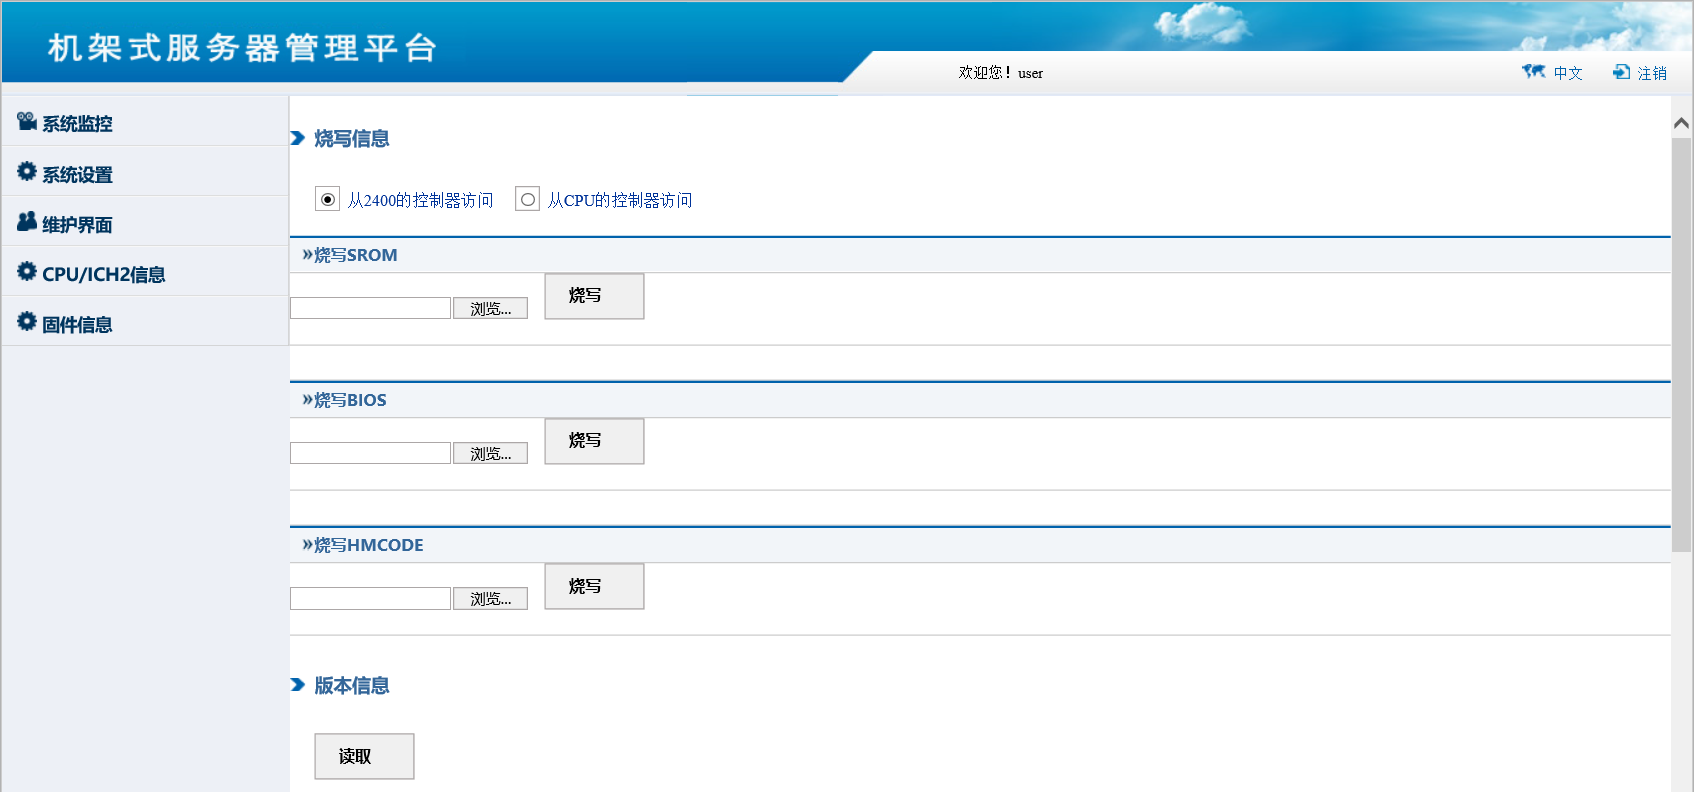
\includegraphics[width=12cm]{bmc.png}
    % 中文标题 %
    \caption*{图 5-4 BMC烧写固件界面}
    % 调整图片英文标题与下文距离(本文标准为-0.7cm) %
    \setlength{\belowcaptionskip}{-0.7cm}
    % 英文标题 %
    \caption*{Fig.5-4 BMC firmware interface}
\end{figure}

然后就是驱动度量日志的查看过程,通过安装的维护工具访问BMC特定端口,并通过linux系统中的重定向输出功能将读取
到的日志信息,写入指定的文件中。图5-7所示为四个特定驱动的度量日志。

\begin{figure}[H]
    % 调整图片与上文的垂直距离 %
    \vspace{0cm}   
    % 调整图片图片与中文标题、中文标题与英文标题距离 %
    \setlength{\abovecaptionskip}{0.3cm}
    % 引用/fig/目录中的图片文件 %
	\centering
    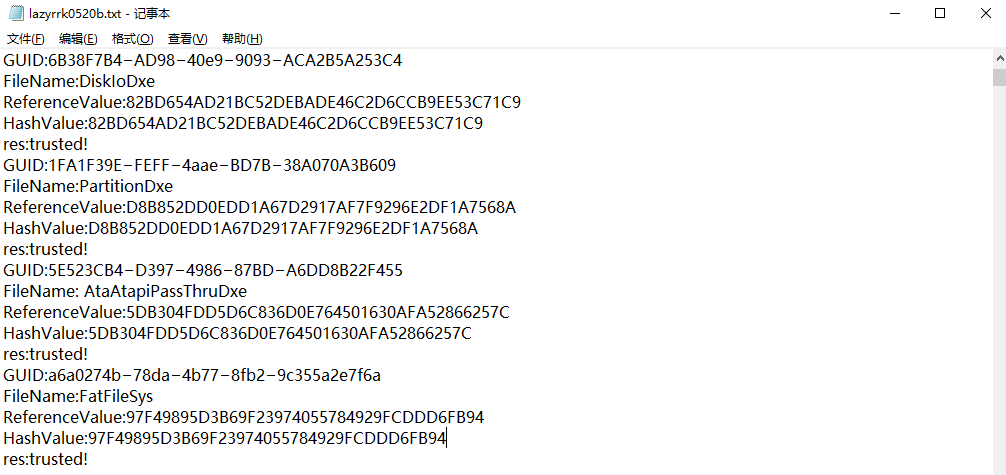
\includegraphics[width=12cm]{log.png}
    % 中文标题 %
    \caption*{图 5-5 驱动度量日志}
    % 调整图片英文标题与下文距离(本文标准为-0.7cm) %
    \setlength{\belowcaptionskip}{-0.7cm}
    % 英文标题 %
    \caption*{Fig.5-5 Driver mesurement log}
\end{figure}

%
% 5.3节
%
\section{BMC驱动连通性实现与测试}
\subsection{功能实现}
\begin{lstlisting}
EFI_STATUS
EFIAPI
IpmiSendCommand (
    IN  EFI_IPMI_INTERFACE_PROTOCOL    *This,
    IN  UINT8                          Command,
    IN  UINT8                          *CommandData,
    IN  UINT8                          CommandDataSize
) {
    ...
    Status = KcsWaitforIbfClear(Instance);
    WriteKcsCommand(Instance,KCS_WRITE_START);
    Status = KcsCheckStatus(Instance,&KcsStatus);
    if(KcsStatus.Bits.State !=KcsWriteState){
    return KcsErrorExit(Instance);
    }
    KcsClearObf(Instance);
    for(i=0; i<DataSize-1; i++) {
        WriteKcsData(Instance,Data[i]);
        Status = KcsCheckStatus(Instance,&KcsStatus);
        if(EFI_ERROR(Status)) {
            return EFI_DEVICE_ERROR;
        }
        if(KcsStatus.Bits.State !=KcsWriteState){
            return KcsErrorExit(Instance);
        }
        KcsClearObf(Instance);
    }
    WriteKcsCommand(Instance,KCS_WRITE_END);
    Status = KcsCheckStatus(Instance,&KcsStatus);
    if(KcsStatus.Bits.State !=KcsWriteState){
        return KcsErrorExit(Instance);
    }
    KcsClearObf(Instance);
    WriteKcsCommand(Instance,Data[i]);
    ...
}
\end{lstlisting}
如上代码所示,通过解析发送命令函数来说明与BMC系统的通信方式。发送函数接收主要的8位标识的命令信息,和命令
数据大小,然后根据IPMI协议提供的KCS数据发送状态流,依次设置KCS命令和查询相关寄存器,配合数据接收寄存器的
数据写入过程\cite{english22}。实现的具体流程参照图4-5。

\subsection{测试目的}
在可信度量驱动程序的开发过程中,需要一个从BMC系统取出基准值的过程,通过单独测试UEFI BIOS中BMC驱动程序
的连通性有助于单独功能地调试可信度量驱动,保证BMC驱动的可用性。

\subsection{测试步骤}
(1)编写DXE阶段的BMC驱动程序,编写BMC的BIOS SHELL命令,可输入IPMI指令和内容,并获取到BMC返回的结果。
将BMC驱动的INF文件添加到申威平台描述文件dsc文件中。
\par (2)然后通过本章第一节中的方法,对申威UEFI组件进行交叉编译。
\par (3)通过BMC提供的烧写功能烧写BIOS固件。
\par (4)服务器上电并按下开机按钮,按F12进入到UEFI界面并通过SHELL启动方式进入到UEFI SHELL环境。
\par (5)输入开发好的BMC命令,并从SHELL界面查看结果。

\subsection{测试过程}
虽然SHELL作为UEFI BIOS系统中的一个上层用户程序,但作为BIOS来说,并不区分内核和用户的内存访问区域,因此
SHELL程序依然可以访问到UEFI初始化的一切系统资源,为驱动的测试提供了基础。

\begin{figure}[H]
    % 调整图片与上文的垂直距离 %
    \vspace{0cm}   
    % 调整图片图片与中文标题、中文标题与英文标题距离 %
    \setlength{\abovecaptionskip}{0.3cm}
    % 引用/fig/目录中的图片文件 %
	\centering
    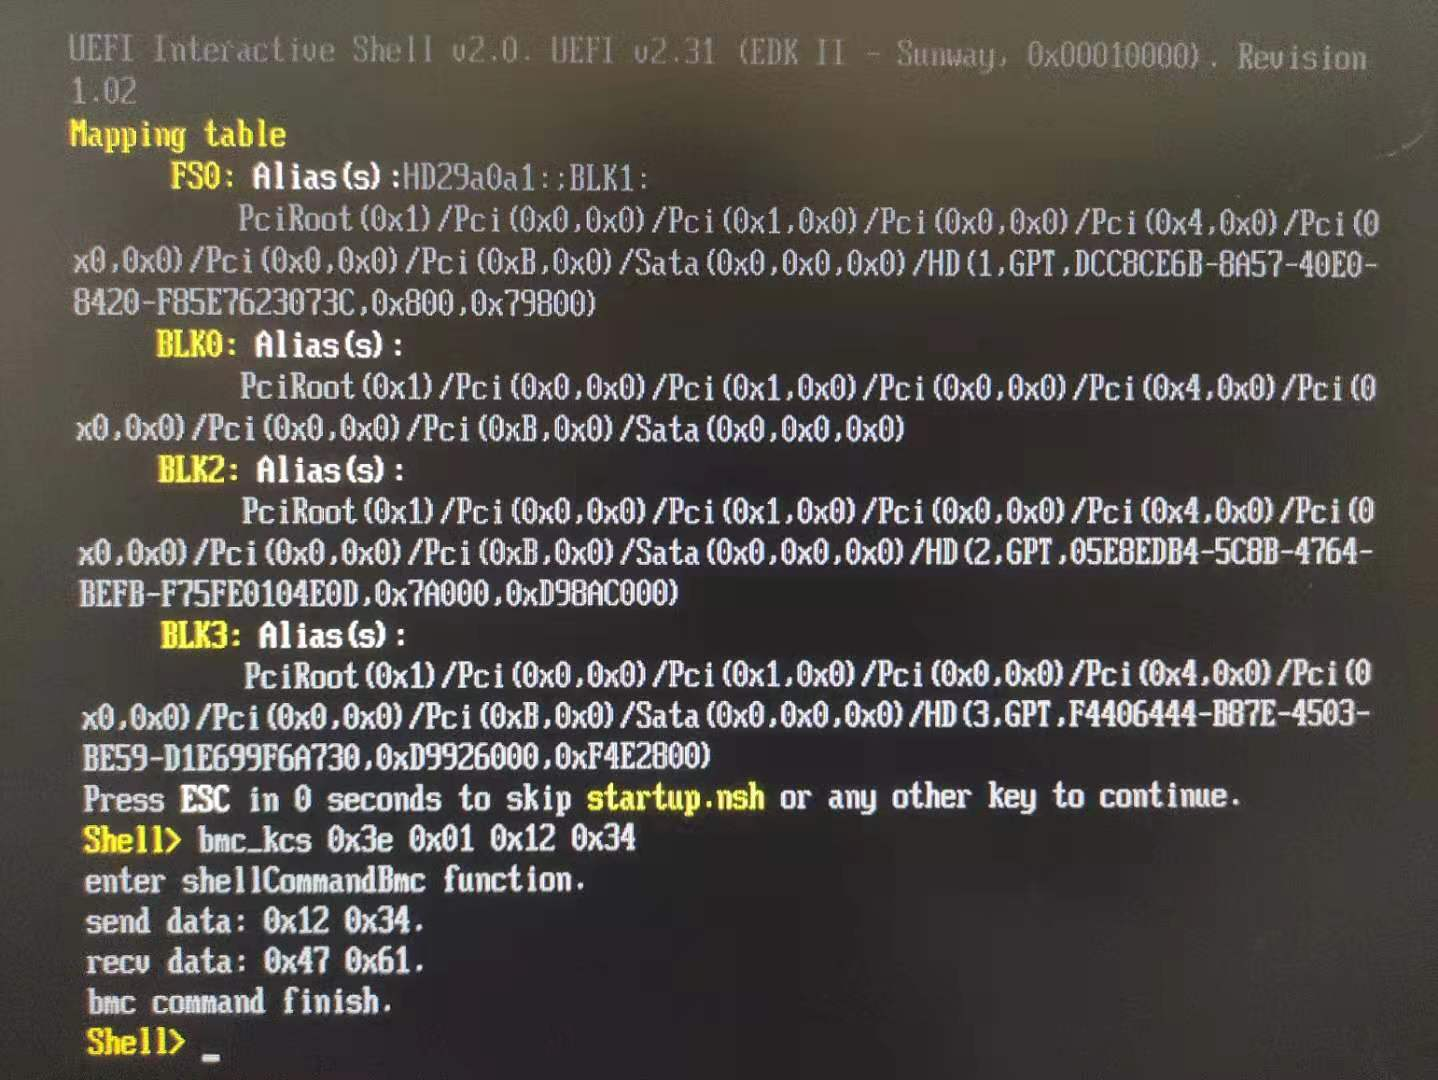
\includegraphics[width=11cm]{bmc_kcs2.png}
    % 中文标题 %
    \caption*{图 5-6 BMC命令运行结果}
    % 调整图片英文标题与下文距离(本文标准为-0.7cm) %
    \setlength{\belowcaptionskip}{-0.7cm}
    % 英文标题 %
    \caption*{Fig.5-6 BMC command results}
\end{figure}

如图5-6所示,是通过名为bmc\_kcs的SHELL命令发送并接收数据的过程。


%
% 5.4节
%
\section{依赖表达式验证}

\subsection{测试目的}
依赖表达式是PEI和DXE驱动加载阶段的加载顺序的主要依据,他与优先级文件对应,属于弱类型。通过验证依赖表达式
在固件文件中的存储以及在驱动加载过程中如何控制加载顺序,可确保可信度量驱动在需被度量的特定驱动前加载,保证
度量功能的可用性。

\subsection{测试步骤}
(1)在DXE core代码的调度器程序中添加向SHELL输出的DEBUG函数。
\par (2)通过配置VS2008来对UEFI BIOS进行编译,得到NT32.fd文件。
\par (3)通过UEFITool这个fd文件解析程序,对NT32.fd进行解析。
\par (4)运行模拟程序的入口点exe可执行文件,根据SHELL输出的DEBUG信息得到依赖表达式解析过程。

\subsection{测试过程}
在经过VS2008编译器编译后生成Windows平台的UEFI模拟环境固件文件,通过UEFITool工具查看到的文件信息如下。

\begin{figure}[H]
    % 调整图片与上文的垂直距离 %
    \vspace{0cm}   
    % 调整图片图片与中文标题、中文标题与英文标题距离 %
    \setlength{\abovecaptionskip}{0.3cm}
    % 引用/fig/目录中的图片文件 %
	\centering
    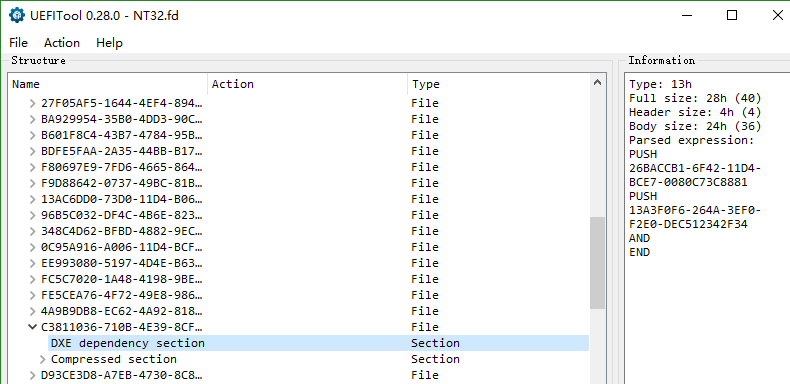
\includegraphics[width=12cm]{fd_depex.png}
    % 中文标题 %
    \caption*{图 5-7 固件文件依赖区域内容}
    % 调整图片英文标题与下文距离(本文标准为-0.7cm) %
    \setlength{\belowcaptionskip}{-0.7cm}
    % 英文标题 %
    \caption*{Fig.5-7 FD file dependency section content}
\end{figure}

图5-8所示的是DXE阶段的TimerDxe驱动在FV格式的固件卷中的dependency section中的内容,两个GUID分别代表两个
协议,他们对应的名称是gEfiCpuArchProtocolGuid和gEfiPcdProtocolGuid。下面是运行过程中TimerDxe驱动对应
的加载过程日志信息显示。

\begin{figure}[H]
    % 调整图片与上文的垂直距离 %
    \vspace{0cm}   
    % 调整图片图片与中文标题、中文标题与英文标题距离 %
    \setlength{\abovecaptionskip}{0.3cm}
    % 引用/fig/目录中的图片文件 %
	\centering
    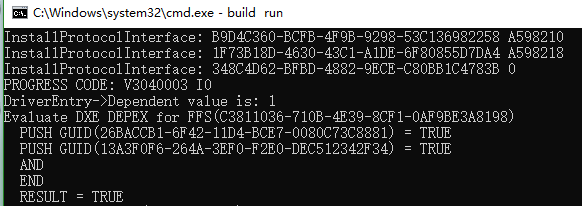
\includegraphics[width=12cm]{timer_depex.png}
    % 中文标题 %
    \caption*{图 5-8 驱动加载过程中的日志信息}
    % 调整图片英文标题与下文距离(本文标准为-0.7cm) %
    \setlength{\belowcaptionskip}{-0.7cm}
    % 英文标题 %
    \caption*{Fig.5-8 Log information during driver loading}
\end{figure}

图5-9显示的是在通过SecMain.exe入口点或命令build run执行后在windows终端里打印显示的BIOS运行过程中的日志
信息,其中可以看到入栈两个协议GUID的过程,并可以看出判断的最终结果为TRUE,在这段log的下方可看到显示了驱动
加载的日志信息。

%
% 5.6节
%
\section{本章小结}
通过三个实验过程的结果可以看出,可信度量驱动具备着从BMC取基准值、生成度量日志和根据依赖表达式定制驱动加载
顺序的功能,这些基本的功能也保证了安全方案的可实现性。

\bjutclearpage
